\subsection{Rete neurale statica}
Il primo strumento che abbiamo utilizzato per lo studio del nostro modello si basa sulle reti di apprendimento di tipo neurale statiche, ovvero il tool Neural fitting di matlab.

Tale tool mette a disposizione dell'utente una semplice GUI la quale permette, attraverso pochi semplici passi di setup, la crezione di una rete neurale statica.

Nonostante tale procedimento sia estramemente semplice, i risultati desiderati possono essere ricavati dopo molte prove dovute a successivi allenamenti della rete ( fase di addestramento ) e a cambiamenti nella struttura interna quali ad esempio il numero di neuroni nascosti.

In particolare la fase di addestramento di una rete neurale prevede che la rete prenda in ingresso un vettore di inputs e ristituisca un risultato, il quale sarà confrontato quindi con un vettore “obiettivo” per verificarne la bontà dei valori ottenuti.

In base all’esito del confronto questa elaborazione viene ripetuta, modificando opportunamente i pesi su ciascun neurone, fino ad ottenere un livello di apprendimento accettabile.

Al fine di ottenere un apprendimento soddisfacente, ovvero che minimizzi l’errore dato dalla differenza tra il vettore obiettivo e il vettore dei risultati ed una retta di regressione il più possibile vicina all'unità, è stato deciso di creare uno script ed una funzione matlab per rendere la ricerca di una rete considerata “ottima” un processo automatico.

Prima di procedere con la spiegazione di tali scripts, è doveroso mostrare quale struttura è stata utilizzata per modellare la rete neurale.

Come possiamo vedere dalla figura sottostante essa prevede uno strato nascosto, composto in linea generale da un numero di neuroni impostabile dall'utente (12 nell'esempio), con funzione di attivazione sigmoide ed uno strato lineare di uscita.

\begin{figure}
  \centering
  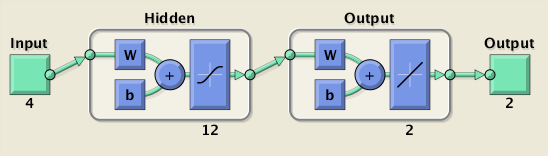
\includegraphics[scale=0.5]{images/neural_net/net.png}
  \caption{Modello di rete neurale}
\end{figure}


\subsubsection{Ricerca della migliore rete neurale}
Nell'ottica di automatizzare il processo di modellizzazione della rete, è stata definita sia una funzione per la ricerca di una rete neurale statica considerata ottima, sia uno script per la visualizzazione dei risultati ottenuti.

\paragraph{Funzione searchBestFitting}
Essa provvede alla creazione di una rete neurale al suo addestramento, e all'estrazione dei parametri di interesse quali il coefficiente della retta di regressione ( nel caso test ) e le performances ( valutate sull'MSE ).
La funzione inizializza, e quindi allena, la rete neurale RETRAIN\_ATTEMPTS volte e restituisce alla fine la migliore rete trovata: ovvero quella che ha presentato nella fase di test i migliori parametri.
Chiaramente sono stati impostati anche due GOALs oltre cui la rete ricavata è considerata ottima, nello specifico si consiedera una rete ottima se i valori di regressione sono maggiori o uguale a 0.99 ed MSE minore di 1000.
Ad ogni passo i parametri discriminanti per la bontà della rete sono quelli della fase di test in quanto indicanti la capacità della rete di generalizzare, e dunque di aver correttamente appreso.
E' importante notare che dopo ogni RETRAIN\_ATTEMPTS la struttura interna della rete viene modificata variando il numero di neuroni dello strato nascosto, in modo da confrontare tra loro diverse configurazioni; infine la funzione di addestramento utilizzata è quella standard di backpropagation di Levenberg-Marquardt (trainlm).
La funzione appena esposta è la seguente:

\inputminted[linenos=true,fontsize=\footnotesize]{matlab}{../../src/neural\ network/functions/searchBestFitting.m}
\captionof{listing}{src/neural network/functions/searchBestFitting.m}


\paragraph{Script netfit}
Tale script si occupa semplicemente di inizalizzare il vettori inputs/outputs, richiamare la funzione appena illustrata e quindi stampare a schermo i risultati ottenuti.
In questo script viene inoltre fatto uso della funzione {\bf unix} di matlab per eseguire lo sript conform.rb per la creazione dei dati necessari alla funzione searchBestFitting.

\inputminted[linenos=true,fontsize=\footnotesize]{matlab}{../../src/netfit.m}
\captionof{listing}{src/netfit.m}


\subsubsection{Risultati}
I risultati ottenuti eseguendo lo script sono i seguenti:

\begin{figure}
  \centering
  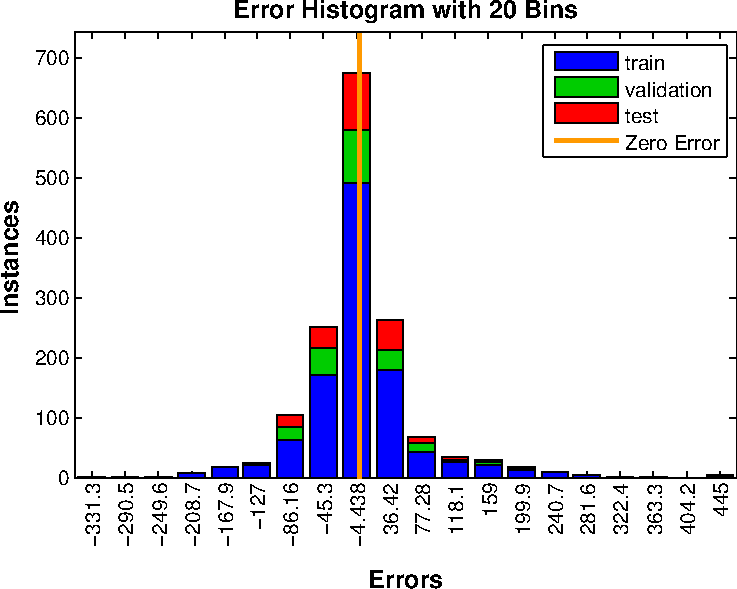
\includegraphics[scale=0.7]{images/neural_net/histogram.pdf}
  \caption{Istogramma degli errori}
\end{figure}

\begin{figure}
  \centering
  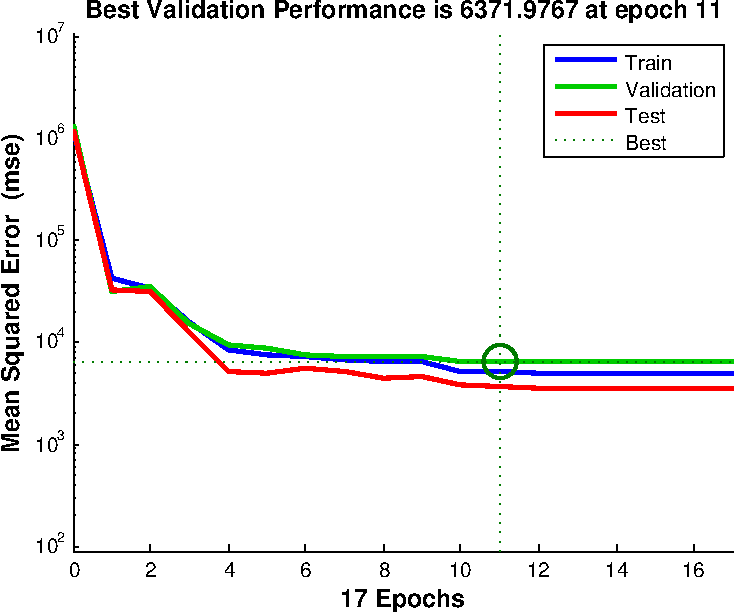
\includegraphics[scale=0.7]{images/neural_net/performances.pdf}
  \caption{Prestazioni della rete (MSE)}
\end{figure}

\begin{figure}
  \centering
  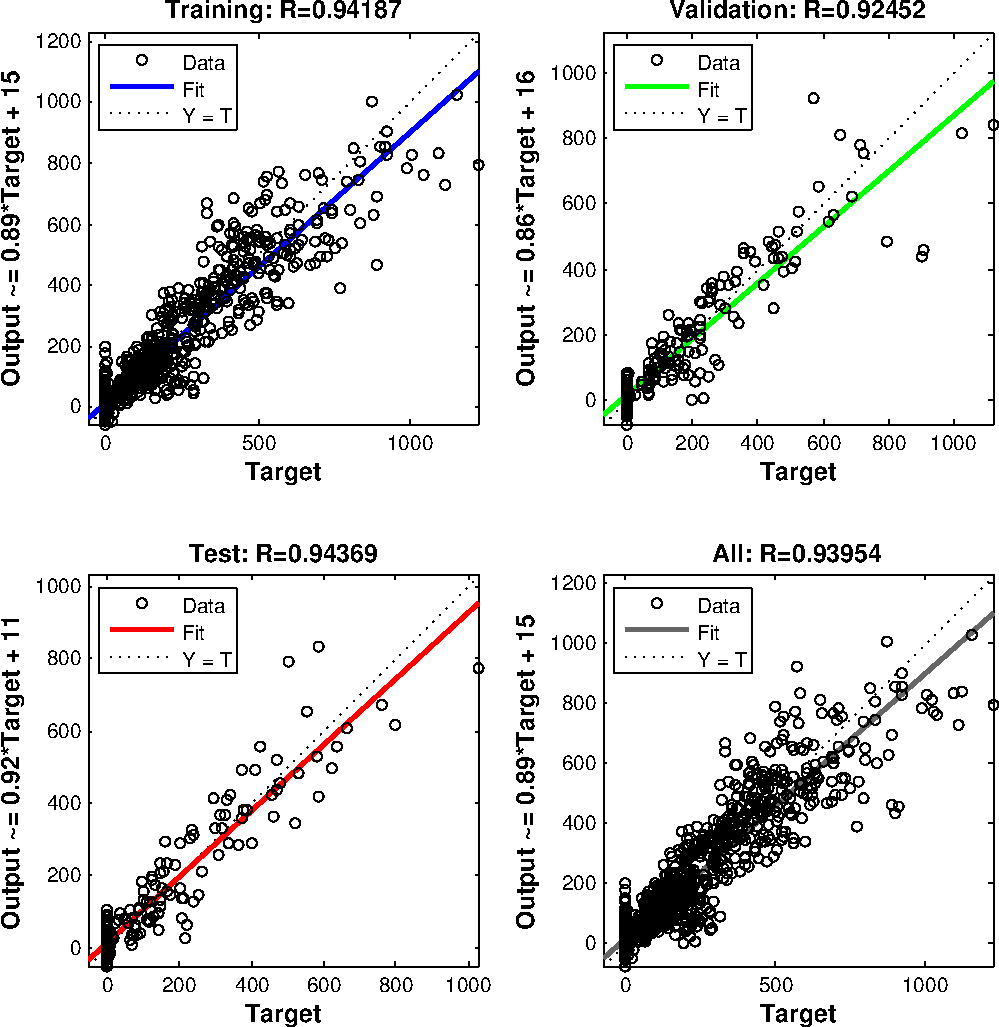
\includegraphics[scale=0.7]{images/neural_net/regressions.pdf}
  \caption{Rette di regressione}
\end{figure}
